\documentclass[12pt]{article}
\usepackage{amsmath}
\usepackage{graphicx}
\usepackage{float}

\usepackage{epsfig}
\usepackage{graphicx}
\usepackage{amsmath}
\usepackage{amsfonts}
\usepackage{amssymb}
\usepackage{amsthm}
\usepackage{longtable}
\usepackage[bf,labelsep=period,textfont=bf,justification=justified,singlelinecheck=false]{caption}
\usepackage[normalem]{ulem}
\usepackage{datatool}
\usepackage[nonumberlist,section=paragraph]{glossaries}
\usepackage{listings}
\usepackage{xcolor}
\usepackage{float}
\usepackage[version=4]{mhchem}
\usepackage{caption}
\usepackage{subcaption}
\usepackage{multicol}
\usepackage[absolute,overlay]{textpos}
\usepackage[export]{adjustbox}
\setlength\columnsep{30pt}

\usepackage[utf8]{inputenc}
\usepackage[english]{babel}

\newtheorem{theorem}{Theorem}

\title{Analytic Tools for the Finite Element Method on Parabolic Equations} 

\author{Geneva Porter, SDSU Spring 2020\\ 
Numerical Partial Differential Equations\\
Dr. Uduak George, Applied Mathematics}

\date{14 May, 2020} 
\begin{document}
\maketitle

The finite element method (FEM) is a technique used to solve many different types of partial differential equations (PDE) on a variety of meshes. Almost always implemented numerically, the FEM has several practical applications in applied mathematics. This report will detail one particular application, solving a time-dependent parabolic reaction-diffusion equation on a surface geometry, and discuss ways in which the theoretical application is valid. The proceeding error analysis will examine the well-posedness, consistency, convergence, and stability of our Schnakenberg Equation model on the surface of a sphere. 

\section{The Surface Finite Element Method}\label{sec:SFEM}

Solving the Schnakenberg equations using the finite element method uses the Laplace-Beltrami operator for a 2D domain in a 3D space. The discretized space is represented numerically by a linear system of matrices, and for parabolic problems, the square matrices are conveniently formatted as symmetric and positive definite. There are several analyses on this process already \cite{Dziuk2012}, so only a brief overview will be given here. 

To begin, the following is the system of differential equations on the 2D surface domain $\Gamma$ embedded in a 3D space:
\begin{equation}
\frac{\partial u}{\partial t} - \Delta_\Gamma u = \gamma~f(u,v) ~~~~~
\frac{\partial v}{\partial t} - \delta\Delta_\Gamma v = \gamma~g(u,v) ~~~~~~ \text{with} ~~~~~~ u = v = 0 ~~ \text{on} ~~ \partial\Gamma
\end{equation}

We treat this as a closed system; therefore there in no flux through the surface. The first step in applying the surface finite element method is to multiply the equations by a test function. The goal of the test function is to give a value to one neighborhood in the discretized domain and return zero for all other neighborhoods. The test function $\varphi$ must satisfy:
\begin{equation}
\varphi\frac{\partial u}{\partial t} - \varphi\Delta_\Gamma u = \varphi\gamma f(u,v) ~~~~~~~ \text{and} ~~~~~~~
\varphi\frac{\partial v}{\partial t} - \varphi\delta\Delta_\Gamma v = \varphi\gamma g(u,v)
\end{equation}

We continue by using the \textit{weak formulation} method by integrating: %For simplicity, the shorthand notation $\int_\Gamma ab = (a,b)$ will be used. 
\begin{equation}\label{eq:weak}
\int_\Gamma \varphi\frac{\partial u}{\partial t} - \int_\Gamma \varphi\Delta_\Gamma u = \int_\Gamma \gamma\varphi f(u,v) ~~~~~~~~~~
\int_\Gamma \varphi\frac{\partial v}{\partial t} - \int_\Gamma \varphi\delta\Delta_\Gamma v = \int_\Gamma \gamma\varphi g(u,v)
\end{equation}

%\begin{equation}
%\label{eq:parenthesis}
%\begin{aligned}
%\longrightarrow ~~~~~ \left(\varphi,\frac{\partial u}{\partial t}\right) - (\varphi, \Delta_\Gamma u) = \gamma~(\varphi, f)  ~~~~~~~~~~ \left(\varphi, \frac{\partial u}{\partial t}\right) - \delta(\varphi, \Delta_\Gamma v) = \gamma~(\varphi, g)
%\end{aligned}
%\end{equation}

Note that we can use integration by parts here, and substitute a more easily computed term for $\Delta_\Gamma$ in this context. Green's Theorem states:
\begin{equation}
\int_{\delta\Gamma} a\cdot\nabla_\Gamma b =  \int_\Gamma a\cdot\Delta_\Gamma b + \int_\Gamma \nabla_\Gamma a \cdot \nabla_\Gamma b
\end{equation}

\noindent Since the flux on the boundary $\partial\Omega$ is zero, we can rewrite (\ref{eq:weak}) as:
%\begin{equation}
%\label{eq:parenthesis2}
%\left(\varphi,\frac{\partial u}{\partial t}\right) + (\nabla_\Gamma\varphi, \nabla_\Gamma u) = \gamma~(\varphi, f)  ~~~~~~~~~~ \left(\varphi, \frac{\partial u}{\partial t}\right) + \delta(\nabla_\Gamma\varphi, \nabla_\Gamma v) = \gamma~(\varphi, g)
%\end{equation}
\begin{equation}\label{eq:weak2}
\int_\Gamma \varphi\frac{\partial u}{\partial t} + \int_\Gamma \nabla_\Gamma\varphi\cdot\nabla_\Gamma u = \gamma\int_\Gamma \varphi f(u,v) ~~~\text{and}~~~
\int_\Gamma \varphi\frac{\partial v}{\partial t} + \delta\int_\Gamma \nabla_\Gamma\varphi\cdot\nabla_\Gamma v = \gamma\int_\Gamma \varphi g(u,v)
\end{equation}

When considering that our domain is not continuous but a mesh of countable elements, we can represent $\Gamma$ as the discretized space $\mathbb{T}$ with elements $K$. In this case, $\mathbb{T}$ is a representation of $\Gamma$ that is partitioned into non-overlapping quadrilaterals. Using this notation, we approximate the system as:
\begin{equation}
\begin{aligned}
\sum_{K\in\mathbb{T}} 
\int_K \varphi\frac{\partial u}{\partial t} + 
\sum_{K\in\mathbb{T}}
\int_K \nabla_K\varphi\cdot\nabla_K u = 
\gamma\sum_{K\in\mathbb{T}}
\int_K \varphi f(u,v) \\
\sum_{K\in\mathbb{T}}
\int_K \varphi\frac{\partial v}{\partial t} + 
\delta\sum_{K\in\mathbb{T}}
\int_K \nabla_K\varphi\cdot\nabla_K v =
\gamma\sum_{K\in\mathbb{T}}
\int_K \varphi g(u,v)
\end{aligned}
\end{equation}

Because our domain is a surface, we must use the tangential gradients when computing the spatial integral (as opposed to the standard gradients for a bulk volume). Recall that the matrices here are symmetric and positive definite. In this context, the tangential gradient is defined for each variable as:
$$\nabla_K u = D\textbf{x}_K G^{-1}_K\nabla u	~~~~~~~~
\nabla_K v = D\textbf{x}_K G^{-1}_K\nabla v$$
$$
\nabla_K \varphi = D\textbf{x}_K G^{-1}_K\nabla \varphi = \nabla \varphi^T G^{-1}_K D\textbf{x}_K^T$$

Furthermore, we can express the spatial elements in terms of a  reference element $\hat{K} = [0,1]^2$, which is beneficial for efficiency in numerical implementation. The reference element is derived from the discretization of the domain mesh. Since our surface mesh is made of quadrilaterals, the reference element will be a unit square. The discretized space can be expressed in terms of the reference element and simplified using the relation $G_k = D\textbf{x}_K^T D\textbf{x}_K$.


\begin{equation}\label{eq:tanint}
\begin{aligned}
&\int_K \nabla_K\varphi\cdot\nabla_K u = \int_{\hat{K}}   \left(\nabla \varphi^T G^{-1}_K D\textbf{x}_K^T\right) D\textbf{x}_K G^{-1}_K\nabla u = \int_{\hat{K}}  \nabla \varphi^T G^{-1}_K  \nabla u   \\
&\int_K \nabla_K\varphi\cdot\nabla_K v = \int_{\hat{K}}  \left(\nabla \varphi^T G^{-1}_K D\textbf{x}_K^T\right) D\textbf{x}_K G^{-1}_K\nabla v = \int_{\hat{K}}  \nabla \varphi^T G^{-1}_K  \nabla v 
\end{aligned}
\end{equation}

% \sqrt{\text{det}(G_k)}

It is prudent to note that this process is referred to as $triangulation$, named from the standard practice in computational mesh generation, which creates surfaces with triangular elements. 



%\begin{equation}
%	\nabla_K u := D\textbf{x}_K G^{-1}_K\nabla u
%	~~~~~~~~~~
%	\nabla_K v := D\textbf{x}_K G^{-1}_K\nabla v 
%\end{equation}

The triangulation process lends itself to numerical representation in vector form. Vertices on the mesh are assigned to positions in a vector, and can be solved as a linear system. With the discretization of space, the variables $u$ and $v$, along with the test function $\varphi$, must in turn be discretized. Below is our discretized approximation for $u$ and $v$, with new variables explained below:
\begin{equation}
u \approx u_K = \sum_j\vartheta_j U_j ~~~~~~~~~~ v \approx v_K = \sum_j\vartheta_j V_j
\end{equation}

We now introduce the basis function $\vartheta_j$. The basis function is similar to the linear algebra standard: a piecewise polynomial whose purpose is to assign a value to a vertex with index $j$, interpolate values for the vertices that share an edge with vertex $j$, and return zero for all other vertices. We create a different basis function for each node on the mesh. In ``classical" FEM formulations, low-degree polynomials are used for each basis function \cite{Tuncer2015}. Predictably, higher degree polynomials result in both increased accuracy and increased computing time. For this thesis, a second degree polynomial will be used for each basis function. $U_j$ and $V_j$ are unknown coefficients, which are treated as variables.

The \textit{deal.ii} library produces a triangulated model with a few simple commands. The use of tangential gradients for surface calculations is more tedious, requiring several nested loops through each vertex on the mesh. 

Our spatially discretized system follows (with the tangential gradient notation omitted for clarity):
\begin{equation}
\begin{aligned}
&\sum_{K\in\mathbb{T}}\sum_j 
\int_K \varphi_i\cdot\vartheta_j\left[\frac{\partial U_j}{\partial t}\right] + 
\sum_{K\in\mathbb{T}}\sum_j
\int_K \nabla_K\varphi_i\cdot\nabla_K \vartheta_j \left[U_j\right] &= 
\gamma\sum_{K\in\mathbb{T}}\sum_j
\int_K \varphi_i f_K(U_j,V_j) \\
&\sum_{K\in\mathbb{T}}\sum_j
\int_K \varphi_i\cdot\vartheta_j\left[\frac{\partial V_j}{\partial t}\right] + 
\delta\sum_{K\in\mathbb{T}}\sum_j
\int_K \nabla_K\varphi_i\cdot\nabla_K \vartheta_j \left[V_j\right] &=
\gamma\sum_{K\in\mathbb{T}}\sum_j
\int_K \varphi_i g_K(U_j,V_j)
\end{aligned}
\end{equation}


With these approximations, the test functions $\varphi_i$ can have a solution for the system at each vertex. For this report, it will be sufficient to state that a unique solution to the above system exists (more on this in future sections). A detailed explanation can be found in \cite{Dziuk2013}, which states that the proof is a direct application of the Lax-Milgram Theorem. For ease of communication, we will simplify the notation here as follows:
$$ \sum_{K\in\mathbb{T}}\sum_j\int_K x\cdot y = \left(\frac{}{}x,y~\right) $$

\noindent Now our system is more easily examined when written as
\begin{equation}\label{eq:simp}
\begin{aligned}
&\left(\frac{}{}\varphi_i,\vartheta_j~\right)\frac{\partial U_j}{\partial t} + \left(\frac{}{}\nabla_K\varphi_i, \nabla_k\varphi_j~\right) U_j &= \gamma \left(\frac{}{}\varphi_i, f_K(U_j, V_j)~\right) \\
&\left(\frac{}{}\varphi_i,\vartheta_j~\right)\frac{\partial V_j}{\partial t} + \delta\left(\frac{}{}\nabla_K\varphi_i, \nabla_k\varphi_j~\right) V_j &= \gamma \left(\frac{}{}\varphi_i, g_K(U_j, V_j)~\right)
\end{aligned}	
\end{equation} 

%Now we must explain the domain on which we will solve. In this case, it is the solid unit sphere. Each discretized cell of the sphere will be a hexahedron. Note that the process forming a discretized mesh in a 3 dimensional space is often called \textit{triangulation}, which can seem misleading, as we are using quadrilateral-faced structures to form the shape mesh (See Appendix \ref{chap:numerical-tools} for the \textit{deal.ii} code that uses the command {\ttfamily triangulation()} for this procedure). The triangulation of the spherical domain is handled using \textit{deal.ii}'s library of basic geometries, which can be refined to more detail an arbitrary number of times (See Appendix \ref{chap:numerical-tools} for more details on \textbf{deal.ii}'s library of geometries). For this theory validation, we will use a spherical mesh refined 5 times, producing a mesh containing $4^5$ hexahedra cells.

Here, it is useful to explain the expansion of the functions $f_K$ and $g_K$, the discretized versions of the reaction equations. Because the solutions are in vector format, we must treat the nonlinear term piecewise; that is, multiply each vector term according to its position in the vector. 

Since the basis functions need only satisfy the linear system, we want it to be as simple as possible. To accomplish this, it is not necessary to create nonlinear terms for the basis function itself. We need only use it in the first degree when attached to the nonlinear term. For example, using $\vartheta_j^3$ as the basis function term for $U_j^2V_j$ is not strictly necessary; using $\vartheta_j$ alone will suffice. In addition, $\alpha$ and $\beta$  are transformed into \textbf{a} and \textbf{b}, which are simply mono-valued vectors corresponding to the size of the basis function vectors. We can now expand the $f_K$ and $g_K$ terms as follows:

\begin{equation}
\begin{aligned}
~&\left(\frac{}{}\varphi_i, f_K~\right)  =& \left(\frac{}{}\varphi_i, \alpha- u_K+ u_K^2v_K~\right)  &= \left(\frac{}{}\varphi_i, \textbf{a} ~\right) - \left(\frac{}{}\varphi_i, \varphi_j ~\right)\cdot U_j + \left(\frac{}{}\varphi_i, \varphi_j ~\right)\cdot U_j^2V_j\\
~&\left(\frac{}{}\varphi_i, g_K~\right)  =& \left(\frac{}{}\varphi_i, \beta- u_K^2v_K~\right) ~~~~ &= \left(\frac{}{}\varphi_i, \textbf{b} ~\right) - \left(\frac{}{}\varphi_i, \varphi_j ~\right)\cdot U_j^2V_j\\
\end{aligned}
\end{equation}

\noindent Note that the notation $U_j^2V_j$ represents the nonlinear term vectors multiplied piecewise. Rewriting Equation (\ref{eq:simp}) using the substitutions above yields:

\begin{equation}\label{eq:simp-full}
\begin{aligned}
&\left(\frac{}{}\varphi_i,\vartheta_j~\right)\frac{\partial U_j}{\partial t} + \left(\frac{}{}\nabla_K\varphi_i, \nabla_k\varphi_j~\right) U_j = \gamma \left[\left(\frac{}{}\varphi_i, \textbf{a} ~\right) - \left(\frac{}{}\varphi_i, \varphi_j ~\right)\cdot U_j + \left(\frac{}{}\varphi_i, \varphi_j ~\right)\cdot U_j^2V_j\right] \\
&\left(\frac{}{}\varphi_i,\vartheta_j~\right)\frac{\partial V_j}{\partial t} + \delta\left(\frac{}{}\nabla_K\varphi_i, \nabla_k\varphi_j~\right) V_j = \gamma \left[\left(\frac{}{}\varphi_i, \textbf{b} ~\right) - \left(\frac{}{}\varphi_i, \varphi_j ~\right)\cdot U_j^2V_j\right]
\end{aligned}	
\end{equation}

We can now use matrix notation for each summation, using the following terms:

\begin{equation*}
\begin{aligned}
\textbf{M} = (\varphi_i,\varphi_j) ~~~~~~~~~~ \textbf{L} = (\nabla\varphi_i, \nabla\varphi_j) ~~~~~~~~~~ \textbf{A} = (\varphi_i,\textbf{a}) ~~~~~~~~~~ \textbf{B} = (\varphi_i,\textbf{b})
\end{aligned}
\end{equation*}

Common nomenclature dictates that \textbf{M} is the mass matrix, \textbf{L} is the Laplace matrix, and \textbf{A} and \textbf{V} are the forcing term vectors. The simple form is now:

\begin{equation}
\begin{aligned}
&\textbf{M}\cdot\frac{d}{dt}[U_j] + \textbf{L}\cdot U_j = \gamma (\textbf{A} - \textbf{M}\cdot U_j + \textbf{M}\cdot U_j^2V_j) \\
&\textbf{M}\cdot\frac{d}{dt}[V_j] + \delta\textbf{L}\cdot V_j = \gamma (\textbf{B} - \textbf{M}\cdot U_j^2V_j)
\end{aligned}
\end{equation}

The spatial discretization is now complete. We can use these results to plug into the temporal discretization, which will be discussed in the next section. We will use the following generalized substitutions:

\begin{equation}\label{eq:space-d}
\begin{aligned}
u \rightarrow \textbf{M}\cdot U_j &~~~~~~~~\ v \rightarrow \textbf{M}\cdot V_j\\
\Delta u \rightarrow -\textbf{L}\cdot U_j &~~~~~~~~ \Delta v \rightarrow -\textbf{L}\cdot V_j\\
\alpha \rightarrow \textbf{A} &~~~~~~~~ \beta \rightarrow \textbf{B} \\	
u^2v &\rightarrow \textbf{M}\cdot U^2_jV_j\\
\end{aligned}
\end{equation}



%%%%%%%%%%%%%%%%%%%%%%%%%%%%%%%%%%%%%%%%%%%%%%%%%%%%%%%%%%%%%%%%%%%%%%%%%%%%%%%%%%%%%%%%%%%%%%%%%%%%%%%%%%%%%%%%%%%%%%%%%%%%%%%%%%%%%%%%%%%%%%%%%%%%%%%%%%%Notes to add to thesis: add details from short explanation on FEM from "Stability, consistency, and convergence" by D Arnold.

\section{Implicit-Explicit Time Stepping Scheme}\label{sec:imex}

The following time discretization will use both implicit and explicit strategies. There is significant evidence that using a combination of implicit and explicit methods improves the stability and decreases the error in temporal discretization schemes \cite{Madzvamuse2006}. Once we assemble the  linear system, we will substitute the spatial discretization terms discussed in Section \ref{sec:SFEM}. To begin, we recall our system of equations:
\begin{equation}
\frac{\partial u}{\partial t} - \Delta u = \gamma~(\alpha - u + u^2v) ~,~~~~~~~~~
\frac{\partial v}{\partial t} - \delta\Delta v = \gamma~(\beta - u^2v)
\end{equation}

\noindent First, let's examine the first equation in terms of $u$. We apply a first order implicit Euler method to the time derivative, with the exception of the nonlinear term. This is one of many forms known as the Implicit-Explicit, or IMEX, discretization scheme. Note that $k$ is the time step length and $N$ is the time step index number.
\begin{equation}
\frac{u_{N+1} - u_{N}}{k} - \Delta u_{N+1} = \gamma~(\alpha - u_{N+1} + u_{N}^2v_{N}) 
\end{equation}

\noindent Separating the unknown values with $u_n$ we get
\begin{equation}
u_{N+1}+k\left(\gamma u_{N+1} - \Delta u_{N+1}\right) = k\gamma\left(\alpha + u_{N}^2v_{N} \right) + u_{N}
\end{equation}


From here, we can solve the equation for $v$ using a slightly more implicit scheme. This is possible because when solving this system numerically, we can solve one equation before the other for each time step. Therefore, the value $u_N$ will be known when solving the equation for $v$. This yields:
\begin{equation}
\frac{v_{N+1} - v_{N}}{k} - \delta\Delta v_{N+1} = \gamma(\beta - u_{N+1}^2v_{N})
\end{equation}

\noindent Again, separating unknown terms yields
\begin{equation}
v_{N+1}-k\left(\delta\Delta v_{N+1}\right) = k\gamma\left(\beta - u_{N+1}^2v_{N} \right) + v_{N}
\end{equation}

\noindent In operator form, the system simplifies to
\begin{equation}\label{eq:time-d}
\begin{aligned}
\left[1 + k\left(\gamma - \Delta\cdot\right)\right]u_{N+1}=  k\gamma\left(\alpha + u_{N}^2v_{N} \right) + u_{N} \\
\left[1 - k\delta\Delta\cdot\right] v_{N+1}=  k\gamma\left(\beta - u_{N}^2v_{N} \right) + v_{N} \\
\end{aligned}
\end{equation}

Using this combination of implicit and explicit approaches allows a moderately high level of accuracy without a significantly complex scheme. We can apply this temporally discretized system to the spatially discretized result of the finite element method linear system by substituting the results to form a linear system. Combining Equation (\ref{eq:time-d}) and the substitutions in (\ref{eq:space-d}), we get:
\begin{equation}
\begin{aligned}
\left[(1+k\gamma)\textbf{M} + k\textbf{L}\right] U_{N+1}&=  k\gamma\left(\textbf{A} + \textbf{M} U^2_{N}V_{N} \right) + \textbf{M}U_{N} \\
\left[\textbf{M} + k\delta\textbf{L}\right] V_{N+1}&=  k\gamma\left(\textbf{B} - \textbf{M} U^2_{N+1}V_{N} \right) + \textbf{M}V_{N} \\
\end{aligned}
\end{equation}

We now have a linear system of the form $\mathcal{A}x=$ \textbf{b}. The $deal.ii$ library has a built-in linear solver, and we utilize the solver's conjugate gradient method for each timestep. For simplicity in further discussion, we will represent the system matrix (left-hand side) and the right hand side matrix as follows:

\begin{equation}
	\mathcal{A} = \left(\begin{matrix} 
	(1+k\gamma)\textbf{M} + k\textbf{L} \\ 
	\textbf{M} + k\delta\textbf{L}
	\end{matrix}\right) ~~~~~
	\textbf{b} = \left(\begin{matrix} 
	k\gamma\left(\textbf{A} + \textbf{M} U^2_{N}V_{N} \right) + \textbf{M}U_{N} \\ 
	k\gamma\left(\textbf{B} - \textbf{M} U^2_{N+1}V_{N} \right) + \textbf{M}V_{N}
	\end{matrix}\right)
\end{equation} 



\section{The Spherical Domain}

Before examining the measures of error for consistency, convergence, and stability, it is useful to establish some details about the domain in question. We will examine an arbitrary pattern on the surface of the sphere for various mesh densities and time step intervals. Each mesh was created using $deal.ii$'s mesh library. In addition, we will be using solution values for $u$ rather than $v$ for the following analyses. The IMEX scheme used grants significantly more accuracy to $v$, so for fairness we will measure the system based on the maximum error.

The mesh itself has a base shape of a cube, and can be refined an arbitrary number of times within a spherical manifold. Upon each refinement, the number of cells in the mesh quadruple, and the maximum diameter among all the cells, $h$, reduces by about half. We will use $h_2$ to denote the maximum diameter after two refinements from a cube, $h_3$ for three refinements, et. cetera. Figure \ref{fig:mesh_density} below shows the four mesh densities we will be working with for the error analysis, while Table \ref{tab:refine} details the numerical information on each mesh, including number of cells and degrees of freedom. Not pictured is the $h_6$ sphere, which will only be used as a domain for an exact solution facsimile.

\begin{figure}[H]\label{fig:mesh density}
	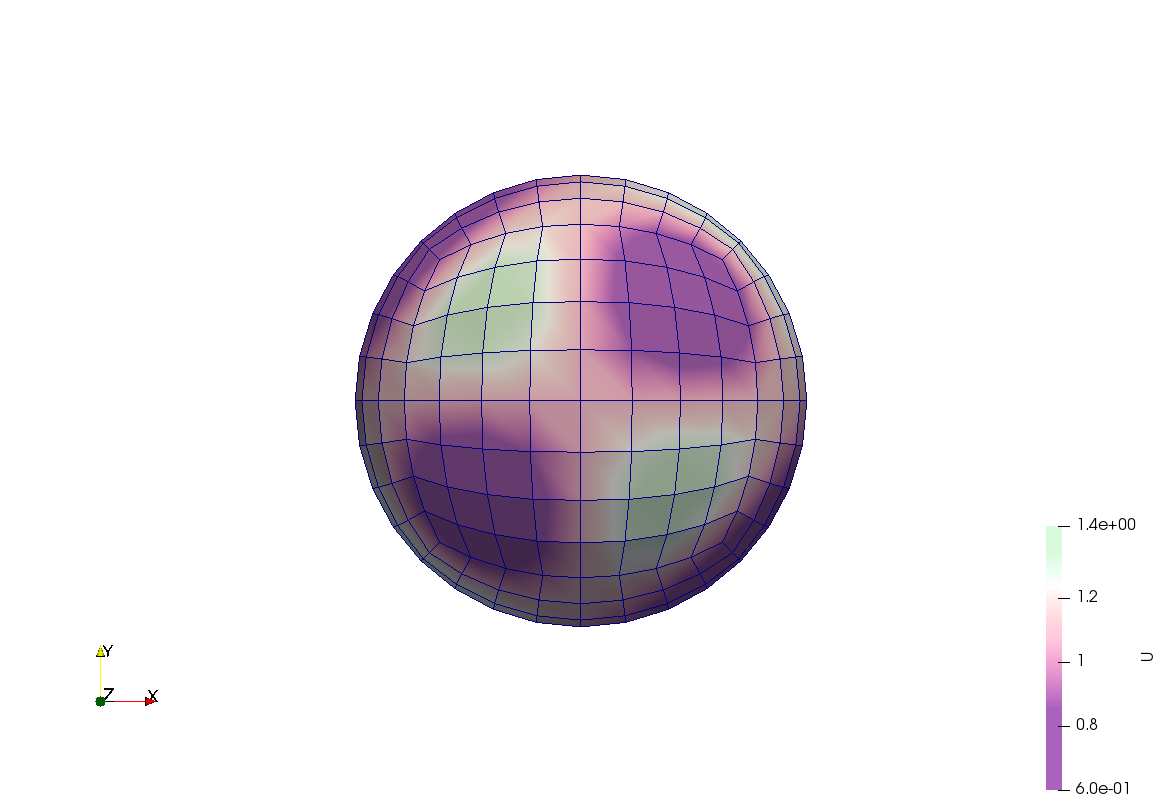
\includegraphics[width=.5\linewidth, trim= 10cm 5cm 10cm 5cm, clip]{images/ref2.png}
	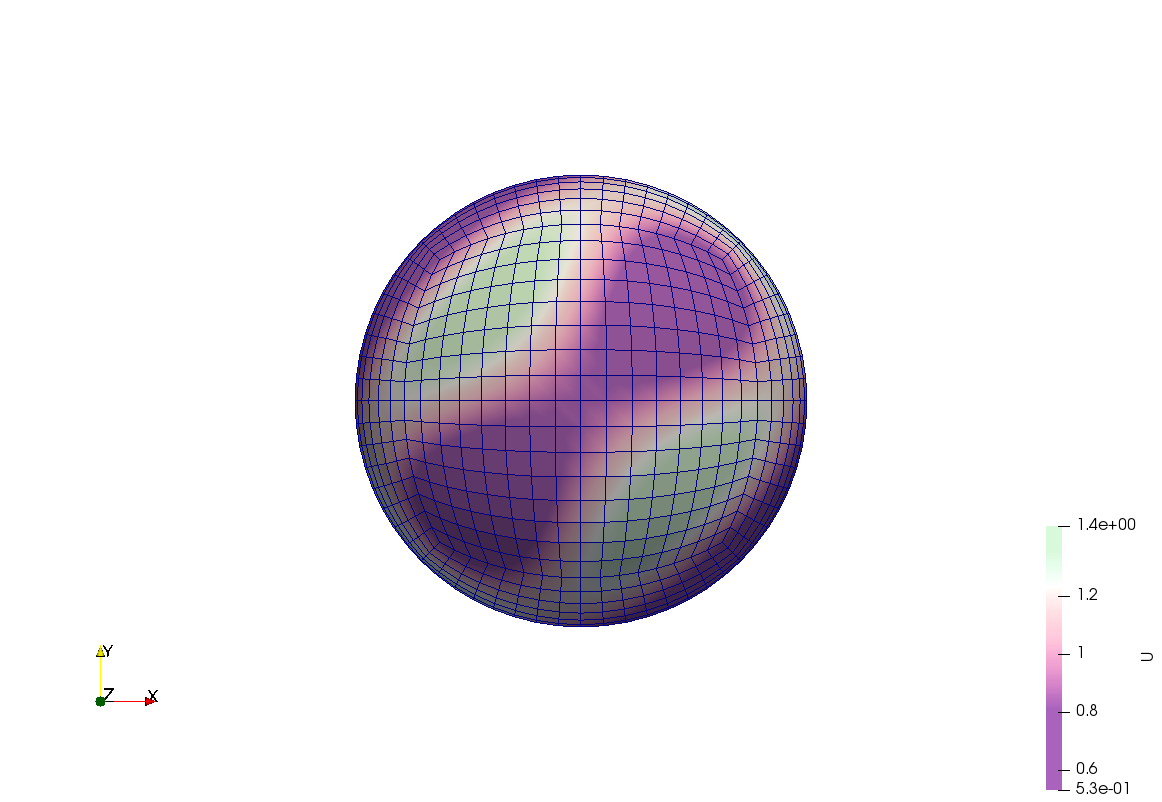
\includegraphics[width=.5\linewidth, trim= 10cm 5cm 10cm 5cm, clip]{images/ref3.png}
	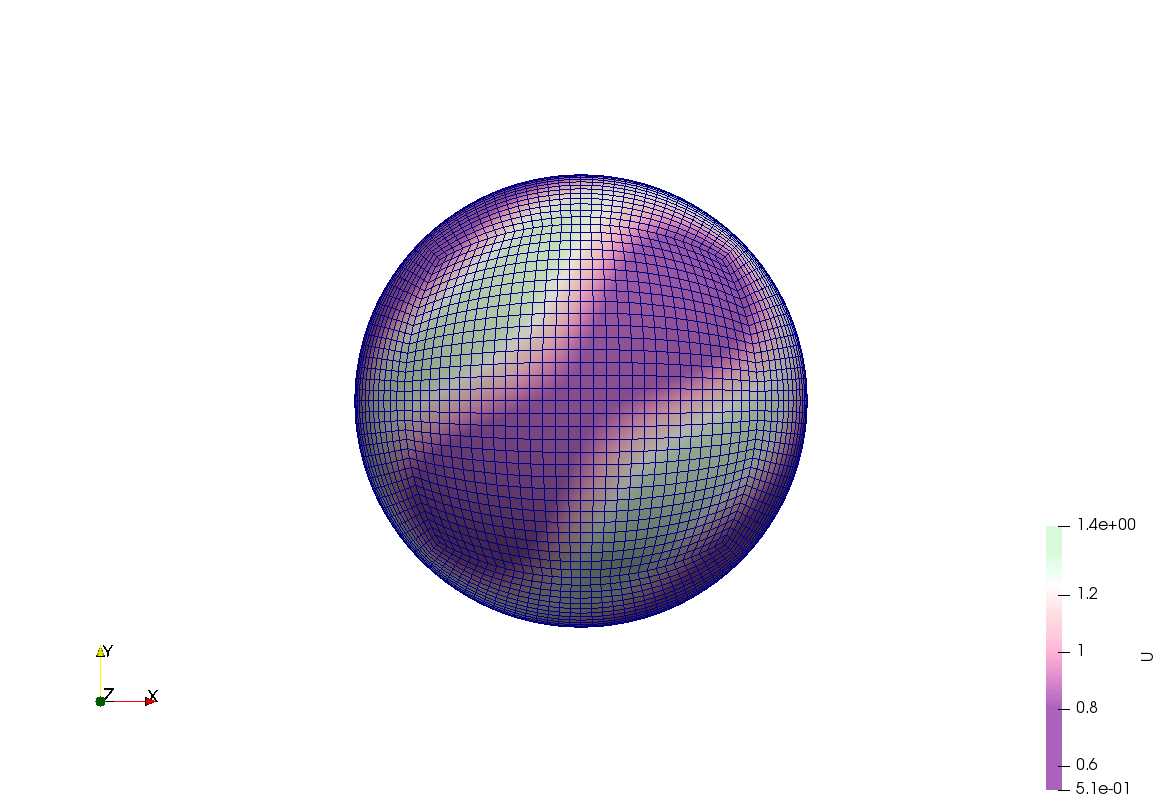
\includegraphics[width=.5\linewidth, trim= 10cm 5cm 10cm 5cm, clip]{images/ref4.png}
	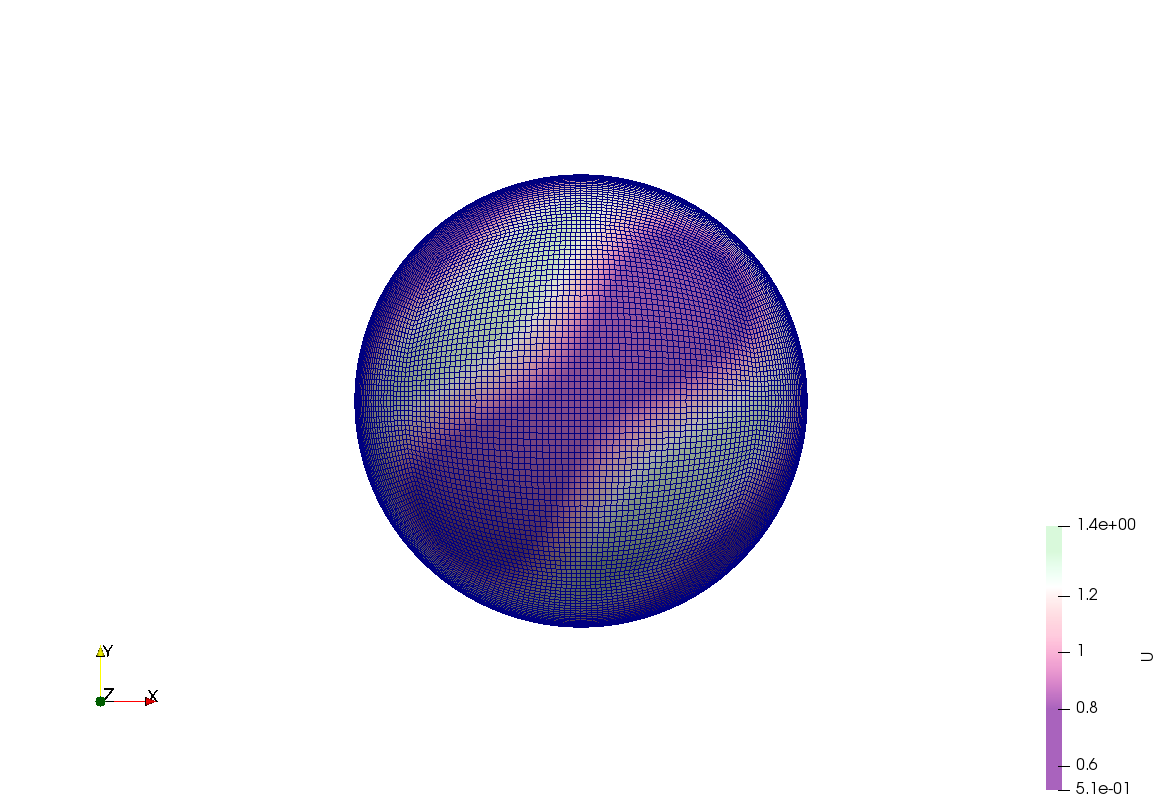
\includegraphics[width=.5\linewidth, trim= 10cm 5cm 10cm 5cm, clip]{images/ref5.png}
	\caption{Sphere meshes with density refinements $h_2$ (top left), $h_3$ (top right), $h_4$ (bottom left), and $h_5$ (bottom right) }\label{fig:mesh_density}
\end{figure}


\begin{table}[H]
	\centering
	\caption{Spherical Mesh Density Values}\label{tab:refine}
	\begin{tabular}{|l|c|c|c|c|c|}
		\hline
		\textbf{}                   & $h_2$    & $h_3$    & $h_4$    & $h_5$     & $h_6$   \\ \hline
		\textbf{Number of Cells}    & 96       & 384      & 1,536    & 6,144     & 24,576\\ \hline
		\textbf{Degrees of Freedom} & 386      & 1538     & 6,146    & 24,578    & 98,306\\ \hline
		\textbf{Maximum Diameter}   & 0.541196 & 0.277048 & 0.139239 & 0.0697337 & 0.034877\\ \hline
	\end{tabular}
\end{table}

Some visualizations to follow only show data up to $t=0.5$. It is important to establish that data collected up to this point is sufficient to show steady-state dynamics. To do this, we will observe a standard L$_2$ norm, as follows:

\begin{equation}\label{eq:norm_standard}
	||u_{N+1} - u_{N}|| = \left(\sum_i^{\dim{u}} (u_{N+1} - u_{N})\right)^2
\end{equation}

Figure \ref{fig:steady-state-h} shows the differences in L$_2$ norms for varying mesh densities, each taken using a timestep length of $10^{-3}$. The norm takes the difference between time steps $u_{N+1}-u_{N}$ as the argument, where $i=1,2,3,...\dim{u}$. We can see that as the mesh density increases (or, as the diameter $h$ halves), the steady state norm value decreases by about half.

\begin{figure}[H]
	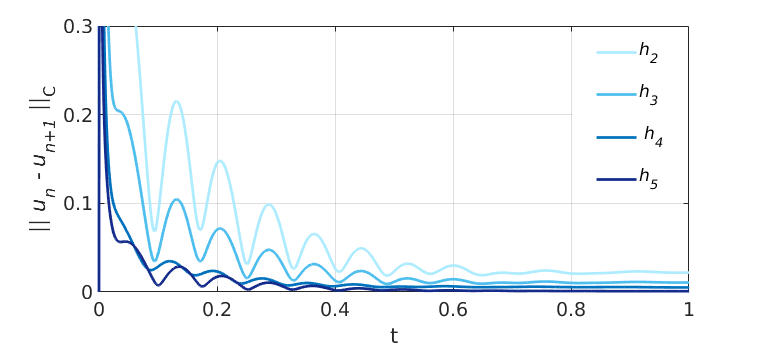
\includegraphics[width=\linewidth]{images/norm_numeric.png}
	\caption{L$_2$ Norm for spheres of various mesh densities.}\label{fig:steady-state-h}
\end{figure}
























\section{Well-Posedness}

We can define a well-posed problem as having three characteristics:

\begin{enumerate}
	\item A solution for the problem exists
	\item The solution is unique
	\item The solution changes continuously as the boundary values and initial conditions change.
\end{enumerate}

To verify that the Schnakenberg system meets these requirements, observe the given equations with their boundary conditions and initial values using the variables $t$, $\phi$, and $\theta$ (note that $r=1$ is constant, since we are only examining the surface):

\begin{equation}
	\begin{aligned}
		\dot{u} - \Delta_\Gamma u = \gamma f(u,v) ~~~~~ f(u,v) = \alpha - u + u^2v ~~~\\
		\dot{v} - \delta\Delta_\Gamma v = \gamma g(u, v) ~~~~~ g(u, v) = \beta - u^2v ~~~ \text{with}\\
		u(t,\pi, \theta) = u(t, -\pi, \theta) ~~~~~ u(t, \phi, \pi) = u(t, \phi, -\pi) \\
		v(t,\pi, \theta) = v(t, -\pi, \theta) ~~~~~ v(t, \phi, \pi) = v(t, \phi, -\pi)	\\
		\text{and} ~~~~~ u_0 = \alpha + \beta ~~~~~ v_0 = \frac{\beta}{(\alpha+\beta)^2}~~~~~~
	\end{aligned}
\end{equation}

This system is a parabolic reaction-diffusion system, which is guaranteed to be well-posed so long as there are at least 2 boundary conditions and the spatial derivative is of the second degree \cite{Tuncer2015}. We can see that there are indeed two boundary conditions and that the spatial derivatives $\Delta_\Gamma u$ and $\Delta_\Gamma v$ are, by definition, of the second degree. We know the system is parabolic because it follows the form:

\begin{equation}
	\begin{aligned}
		A_1u_{xx} + 2B_1u_{xt} + C_1u_{tt} + D_1u_x + E_1u_t + F_1 = 0 \\
		A_2v_{xx} + 2B_2v_{xt} + C_2v_{tt} + D_2v_x + E_2v_t + F_2 = 0
	\end{aligned}
\end{equation}

Here, the spatial derivatives $\Delta_\Gamma u$ and $\Delta_\Gamma u$ are represented by $u_{xx}$ and $v_{xx}$, respectively. The time derivatives $\dot{u}$ and $\dot{v}$ are likewise represented by $u_t$ and $v_t$. For both equations, the coefficients corresponding to $B$ and $C$ are equal to zero, so the criteria for parabolic classification $B^2-AC=0$ is met. Since the problem is well-posed, we can continue to make other important inferences later on.


























\section{Consistency}

For FDM, consistency occurs when mesh cells and time step size decrease, the truncation error approaches zero. In other words, the discrete system should be a ``good" approximation of the partial differential equation system. Normally we would determine consistency by showing:

\begin{equation}
	P\phi - P_{k,h}\phi \rightarrow 0 ~~~\text{as} ~~~ k,~h \rightarrow 0
\end{equation}

However, for nonlinear time dependent PDEs, we can measure consistency by examining the local truncation error \cite{Bonito2010}. For the system in question, we solve each time step via a linear equation. Recall the linear system we set up using the FEM-IMEX scheme:

\begin{equation}
	\mathcal{A}x=\textbf{b}
\end{equation}

\noindent Here $x=(u^{N+1}, v^{N+1})^T$, and \textbf{b} is a function of $(u^N, v^N)$. To find the truncation error, we apply a simple check after solving the system:

\begin{equation}\label{norm}
	\text{Truncation error} = ||\textbf{b}-\mathcal{A}x|| 
\end{equation}

The truncation error is already an integral part of the algorithm for solving the linear system (in this case, the conjugate gradient method). We can apply a constraint that forces the solver to continue enumerating until the solution gives a truncation error below the desired amount. This feature also allows us to easily control the accuracy to order $p$, so long as we constrain the truncation error as being less than both $\mathcal{O}(k^p)$ and $\mathcal{O}(h^p)$. 

We define order $p$ by the following inequality:

\begin{equation}
	||\textbf{b}-\mathcal{A}x|| \lessapprox h^{p_1}+k^{p_2}
\end{equation}

We can then say that the numerical scheme is consistent if it is accurate of order $p=(p_1,p_2)>0$. For this analysis, we constrained the conjugate gradient algorithm to iterate until the truncation error was less than $10^{-20}$. Therefore, we can achieve an arbitrarily high accuracy order so long as we are willing to sacrifice the computing time needed to achieve it. Since we keep the truncation error at $10^{-20}$ for all computational runs, all permutations of $h$ and $k$ in the proceeding analysis are consistent with an order of accuracy of at least (2,2). 























\section{Convergence}

While consistency examines the discretization of a system, convergence implies that the $solution$ to the discrete system is a ``good" approximation to the $solution$ of the partial differential equation system. Now, we cannot measure convergence in the traditional way, because it requires knowledge of the exact solution. The exact solution to the Schnakenberg system on the surface of a spherical domain in unknown. However, we can create a facsimile of the exact solution by producing an output using the smallest time step and cell size that is computationally feasible. 

If we call this exact solution facsimile $W_E$ while our approximate solution is $W_h$, then we can say that the solution converges given that the following criteria is satisfied:

\begin{equation}
\left|\left|\frac{}{} W_h - W_E ~\right|\right| \lessapprox h^{q_1} + k^{q_2} 
\end{equation}

However, because of computational limitations, it was not feasible to calculate the difference $W_h-W_E$ for each time step. Instead, we examined the convergence rate based on the following inequality:

\begin{equation}
\left|\frac{}{} ||W_h|| - ||W_E|| ~\right| \leq \left|\frac{}{} || W_h - W_E|| ~ \right|  \lessapprox \left|h^{q_1} + k^{q_2}\right| = h^{q_1} + k^{q_2}
\end{equation}

\noindent Using $\left|\frac{}{} ||W_h|| - ||W_E|| ~\right|$ is a valid measure so long as $q=(q_1,q_2) > 0$, then the solution converges at rate $q$. The norms are the same as the one defined in (\ref{eq:norm_standard}). We can also show this graphically. Figure \ref{fig:convergence} below shows how the convergence rates change for varying $h$ and $k$. Note that each successive graph (from right to left) is zoomed in by a factor of 10 for the $y$-axis.

\begin{figure}[H]
	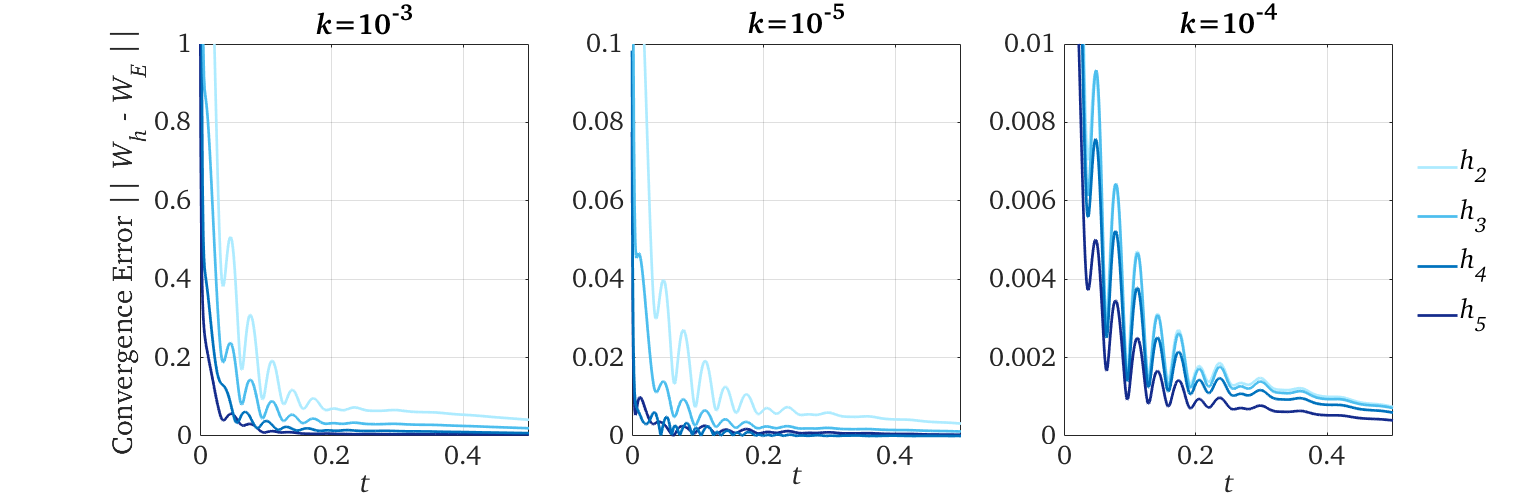
\includegraphics[width=\linewidth, trim=2.5cm 0 .5cm 0,clip]{images/norms_1.png}
	\caption{Convergence norms for varying $h$ and $k$}\label{fig:convergence}
\end{figure}

Convergence norm values are shown in Table \ref{tab:converg_norms} below, for various values of $h$ and $k$. Table \ref{tab:converg_rates} shows the maximum convergence rate for each pair of values $(h,k)$. We can confidently say that all models converge to some degree. Note that convergence rates steadily increase as $k$ decreases.

\begin{table}[H]
	\caption{Convergence Norm Values For Various $h$ and $k$}\label{tab:converg_norms}
	\centering
	\begin{tabular}{|l|l|l|l|l|}
		\hline
					& $h_2$  & $h_3$  & $h_4$  & $h_5$  \\ \hline
		$k=10^{-3}$ & 1.9e-3 & 1.3e-3 & 5.0e-3 & 1.0e-2 \\ \hline
		$k=10^{-4}$ & 1.8e-4 & 1.2e-4 & 4.9e-4 & 1.0e-3 \\ \hline
		$k=10^{-5}$ & 1.8e-5 & 1.2e-5 & 4.9e-5 & 1.0e-4 \\ \hline
	\end{tabular}
\end{table}


\begin{table}[H]
	\caption{Convergence Rates For Various $h$ and $k$}\label{tab:converg_rates}
	\centering
	\begin{tabular}{|l|l|l|l|l|}
		\hline
		            & $h_2$    & $h_3$  & $h_4$    & $h_5$  \\ \hline
		$k=10^{-3}$ & (10, 10) & (5, 5) & (2, 2)   & (1, 1) \\ \hline
		$k=10^{-4}$ & (14, 14) & (7, 7) & (3, 3)   & (2, 2) \\ \hline
		$k=10^{-5}$ & (17, 17) & (8, 8) & (5, 5)   & (3, 3) \\ \hline
	\end{tabular}
\end{table}


\section{Stability}

Stability in a finite difference system demands that the solution is persistent, that is, small perturbations or errors (such as round-off errors) in the data disappear over time. In addition, it implies that a change of the initial and boundary data leads to a comparable change in the numerical solution. This concept is identical for the finite element method. In fact, the formal definition tells us that our solution $must$ be stable, since it is consistent and converges \cite{MurrayII2003}:

\begin{theorem}[Lax-Richtmyer]
	Let $W_h$ be the solution of a numerical method consistent with a well-posed time-dependent problem; in particular, assume that it is accurate of order $p>0$. Then, if the numerical method is stable, its solution converges with $p$th-order convergence rate,
	$$\left|\left|\frac{}{} W_h - W_E~\right|\right| \lessapprox \sum_{m=0}^n k\cdot ||\textbf{b}-\textbf{A}x|| \lessapprox h^{p_1} + k^{p_2}, ~~~t^n\in[0,T].$$
\end{theorem}

We have shown that the system and solution is consistent and convergent. Therefore, the FEM-IMEX approach is stable. We can confidently use this model for research into other applications.


\bibliographystyle{unsrt}
\bibliography{bib_all}

\end{document}


































We can now show that we achieved consistency, with of accuracy order (2,2), by graphically examining a few items of data collected when solving on a sphere. Each spatial refinement of the sphere doubled the number of cells and decreased the cell diameter by half. We proceeded by evaluating the following comparisons:


\begin{enumerate}
	\item Plotting the local error vs. each time step for $t<1$ for various $k$, repeat plot for various $h$
	\item Plotting local error at steady state for $t=1$ vs. $k$ for various $h$
	\item Creating a table showing the elements that ensure accuracy of order 2.
\end{enumerate}

For the following plots, we will examine the solutions for $u$ only. Because of the way the IMEX scheme is implemented, $v$ is slightly more accurate, so we will perform our analysis at a measure of maximum error. First let's examine the truncation error for $k=10^{-2}$, $10^{-3}$, $10^{-4}$, and $10^{-5}$ for $h_3$. We can then repeat the analysis for $h_4$ and $h_5$. Figures \ref{fig:h3_consistency}, \ref{fig:h4_consistency}, and \ref{fig:h5_consistency} below show these plots.


\begin{figure}[H]
	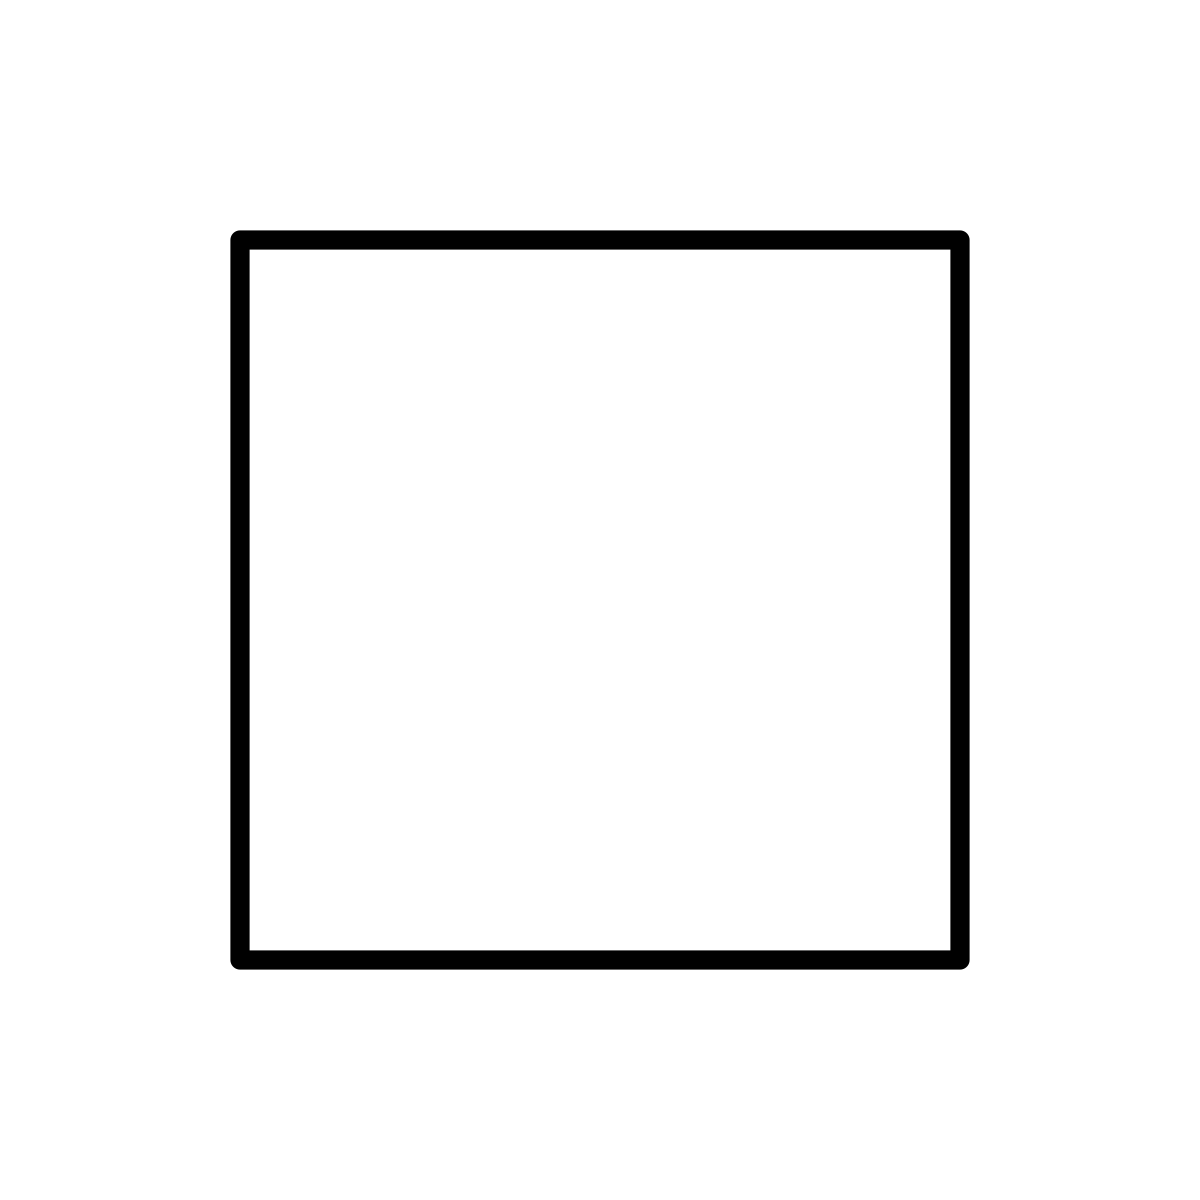
\includegraphics[width=\linewidth]{xxx.png}
	\caption{Consistency plot for $h_3$ at various time steps $k$.}\label{fig:h3_consistency}
\end{figure}

\begin{figure}[H]
	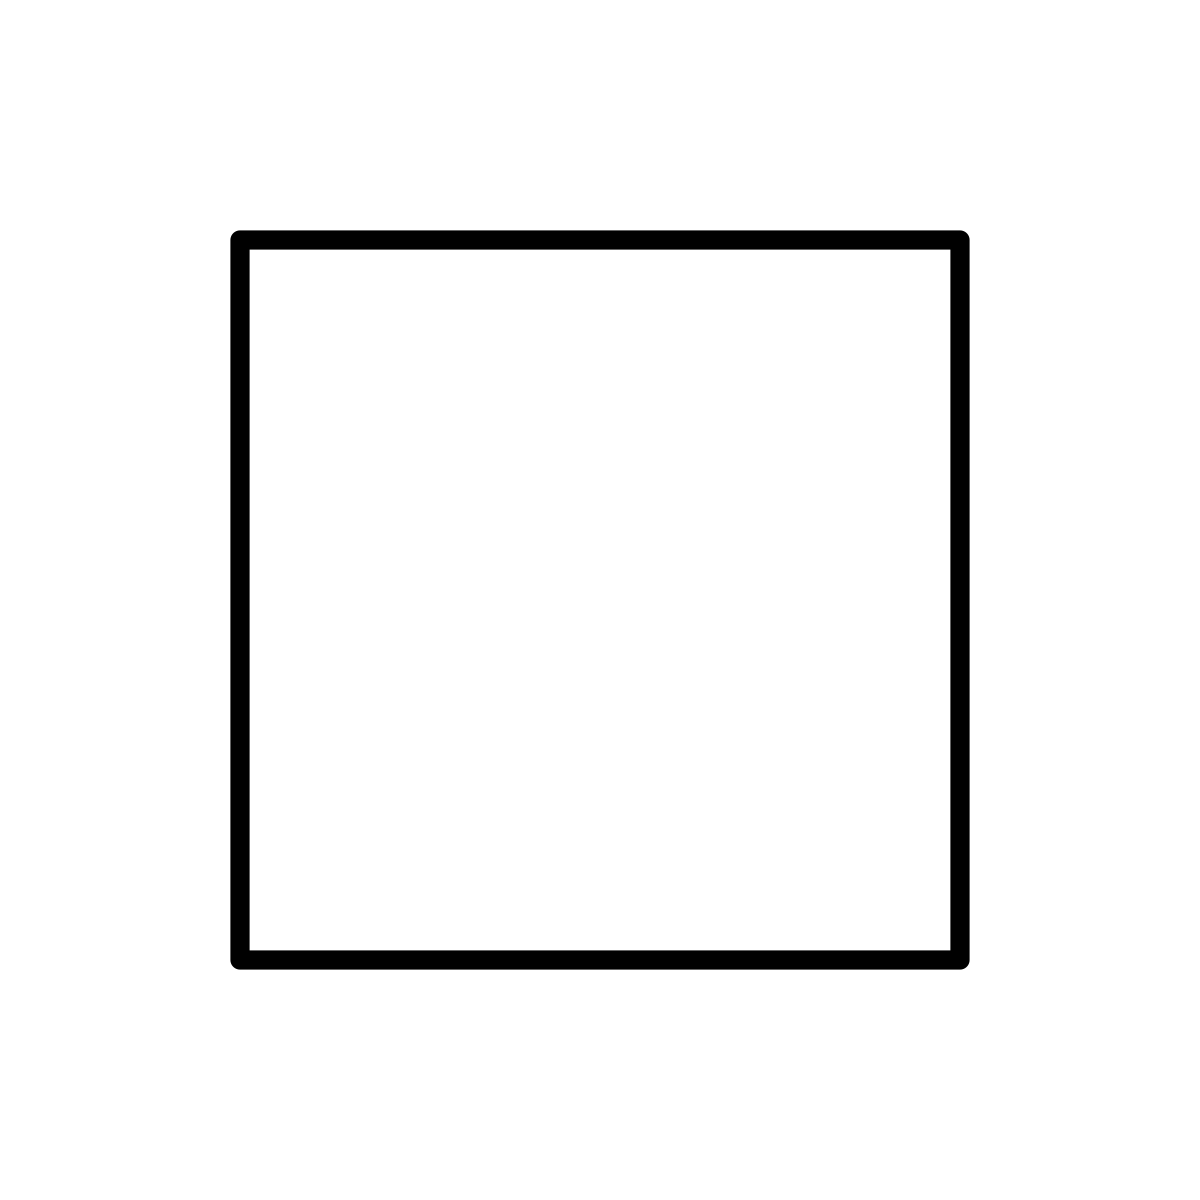
\includegraphics[width=\linewidth]{xxx.png}
	\caption{Consistency plot for $h_4$ at various time steps $k$.}\label{fig:h4_consistency}
\end{figure}

\begin{figure}[H]
	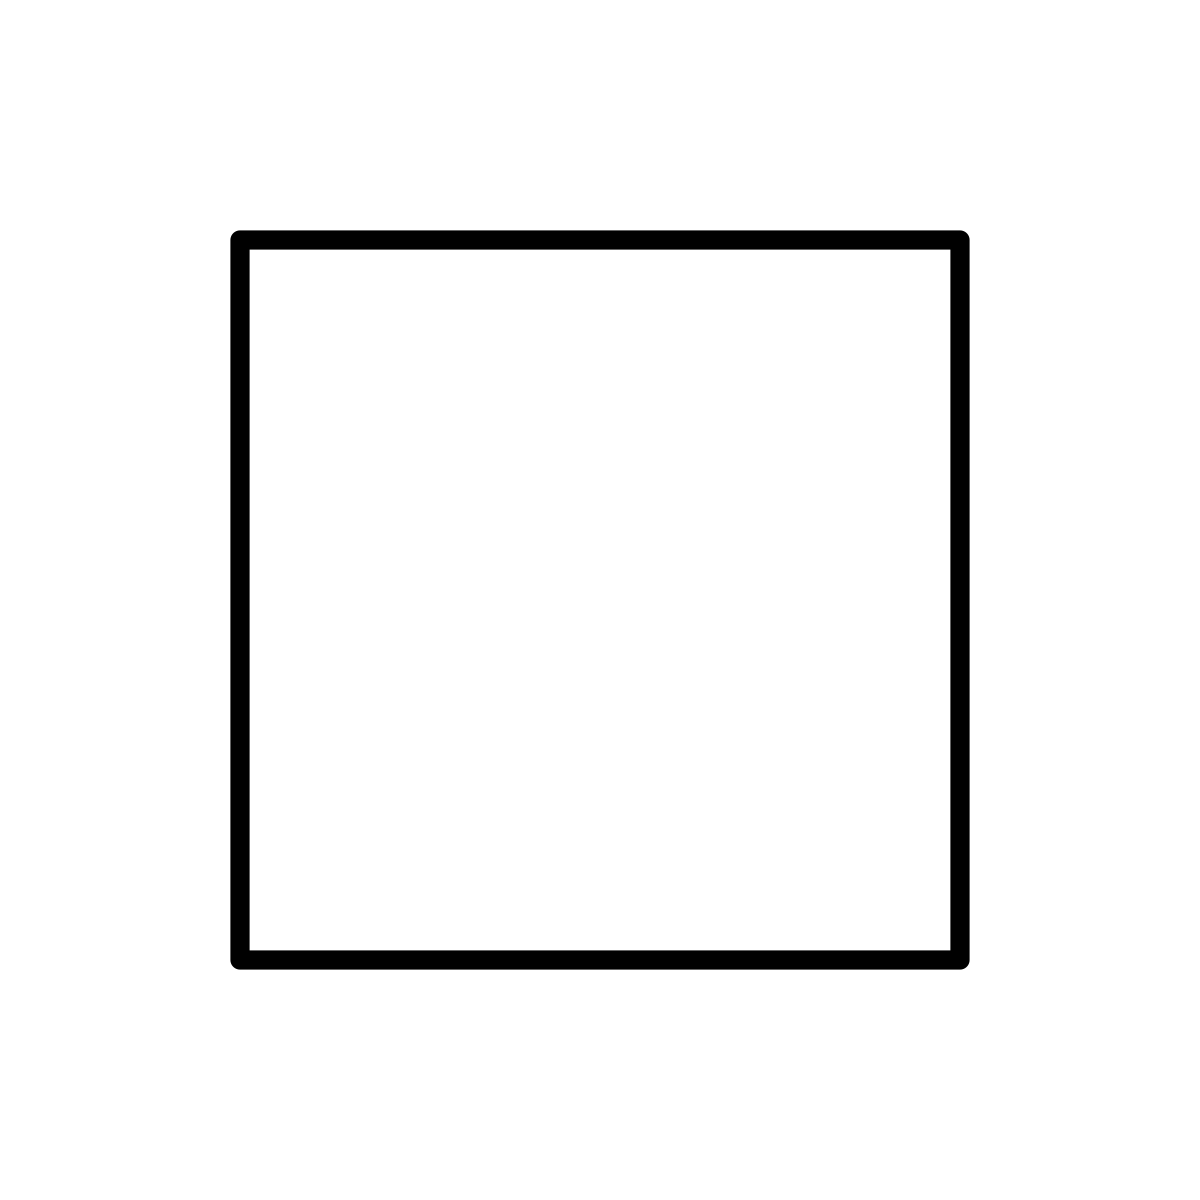
\includegraphics[width=\linewidth]{xxx.png}
	\caption{Consistency plot for $h_5$ at various time steps $k$.}\label{fig:h5_consistency}
\end{figure}

We can now show that the consistency order increases as $k$ and $h$ decrease. Figure \ref{fig:k_consistency} shows the changes in the consistency curve at the steady-state as both $k$ and $h$ decrease.








Another way to verify that the problem is well-posed is to apply the Lax-Milgram Theorem. 

\begin{theorem}[Lax-Milgram]
	Let $V$ be a Hilbert space and a(.,.) a bilinear form on V, which is 
	\begin{enumerate}
		\item bounded: $|a(u,v)| \leq C ||u||~||v||$ and
		\item coercive: $a(u,u) \geq ||u||^2$.
	\end{enumerate}
	Then, for any $f \in V'$, there is a unique solution $u\in V$ to the equation $a(u,v)=f(v)  \forall v \in V$, and it holds $||u|| \leq \frac{1}{c} ||f||_{V'}$.
\end{theorem}

Recall the weak formation FEM step. The Lax-Milgram Theorem














